\documentclass[14pt]{extarticle}
\usepackage{fontspec}
\usepackage{geometry}
\geometry{a4paper, margin=2.1cm}
\usepackage{graphicx}
\usepackage{booktabs}
\usepackage{array}
\usepackage{amsmath}
\usepackage{amssymb}
\usepackage[table]{xcolor}
\usepackage{titlesec}
\usepackage{fancyhdr}
\usepackage{enumitem}
\usepackage[most]{tcolorbox}

\definecolor{theme}{HTML}{2b6a77}
\definecolor{ink}{HTML}{232d33}
\definecolor{ok}{HTML}{3f8161}
\definecolor{warn}{HTML}{b5651d}
\definecolor{cardbg}{HTML}{f3f6f7}
\definecolor{softgray}{HTML}{eef1f2}

\setmainfont{THSarabunNew.ttf}[
  Path=./fonts/, BoldFont=THSarabunNew Bold.ttf,
  ItalicFont=THSarabunNew Italic.ttf, BoldItalicFont=THSarabunNew BoldItalic.ttf]
\setmonofont{cour.ttf}[Path=./fonts/, BoldFont=courbd.ttf, Scale=0.82]
\XeTeXlinebreaklocale "th"
\XeTeXlinebreakskip = 0pt plus 0.1pt

\titleformat{\section}{\Large\bfseries\color{theme}}{\thesection.}{0.5em}{}
\titleformat{\subsection}{\large\bfseries\color{ink}}{\thesubsection}{0.5em}{}
\setlist{itemsep=1pt, topsep=2pt}
\pagestyle{fancy}\fancyhf{}
\fancyhead[L]{\small\color{ink} CL-1 · Statistical Convergence \& Power}
\fancyhead[R]{\small\color{ink}\thepage}
\renewcommand{\headrulewidth}{0.4pt}
\newcommand{\code}[1]{{\ttfamily\detokenize{#1}}}
\newtcolorbox{keybox}{colback=cardbg, colframe=theme!55, boxrule=0.8pt, arc=2pt, left=8pt, right=8pt, top=5pt, bottom=6pt}

\begin{document}

\begin{center}
{\LARGE\bfseries\color{theme} รายงานการทดสอบสมมติฐาน CL-1}\\[3pt]
{\Large Statistical Convergence \& Power}\\[5pt]
{\small การตรวจจับรอยแตกด้วยลายเซ็นการกระเจิง (SPR) --- OpenGATE 10 / Geant4}\\
{\small รายงานเฉพาะการทดสอบ CL-1 \quad$\bullet$\quad \today}
\end{center}
\vspace{2pt}{\color{theme!45}\hrule}\vspace{8pt}

\section*{บทคัดย่อ}
CL-1 ทดสอบว่า ``การเพิ่มสถิติจะยืนยันการตรวจพบรอยแตกเล็กสุด (0.306~มม.) และคลี่คลายภาวะอิ่มตัว
(plateau) ระหว่าง 0.54 กับ 1.0~มม. ได้หรือไม่'' รายงานนี้วิเคราะห์ \textbf{การลู่เข้า (convergence),
ช่วงความเชื่อมั่นแบบ bootstrap, และการวิเคราะห์กำลัง (power)} บนข้อมูล 8 seeds จาก CL-0 ผลสรุป:
(1)~\textbf{การตรวจพบทั้งสี่ขนาด robust} --- ช่วงความเชื่อมั่น 95\% ของ $\Delta$SPR ตัดค่า 0 ทุกขนาด;
(2)~\textbf{0.306~มม.\ ยืนยันแล้วด้วยการรันจริง} --- เดิมก้ำกึ่งที่ $N=8$ ($p=0.017$), รันเพิ่มเป็น $N=30$
ได้ \textbf{$p=0.00004$} ($t=-4.86$, reliability 99\%) $\Rightarrow$ ตรวจพบรอยแตกเล็กสุดอย่างเด็ดขาด;
(3)~\textbf{plateau แยกไม่ออกทางสถิติ} ($p=0.48$) และการแยก 0.54/1.0 ด้วย ROI-mean ต้องใช้
ถึง $\sim$111 seeds --- \textbf{การเพิ่ม seed จึงไม่ใช่วิธีที่คุ้มสำหรับ plateau ควรเปลี่ยนไปใช้ตัวชี้วัด
เชิงพื้นที่ (CL-7)} แทน

\section{สมมติฐานและขอบเขต}
\textbf{สมมติฐาน CL-1:} ถ้าสัญญาณจริง การเพิ่ม $N_{\text{seeds}}$/$N_{\text{photons}}$ จะทำให้ $|t|$ โตขึ้น
อย่างเสถียร $\Rightarrow$ (ก)~ยืนยัน 0.306~มม.\ ให้พ้นความก้ำกึ่ง และ (ข)~ชี้ขาดว่า plateau เป็นของจริง
หรือเป็นเพียง noise\\
\textbf{ข้อมูลที่ใช้:} ผล 8 seeds ต่อขนาดจาก CL-0 (matched control, collimated, a-priori ROI 16$\times$16px)
--- วิเคราะห์เชิงลึกโดยไม่ต้องรันใหม่ ก่อนตัดสินใจลงทุนรันสถิติสูง (ดู \S\ref{sec:next})

\section{วิธีวิเคราะห์}
\begin{enumerate}
  \item \textbf{Cumulative-seed convergence:} คำนวณ $t$ โดยใช้ seed สะสม $n=2,\dots,8$ เพื่อดูการลู่เข้า
  \item \textbf{Bootstrap} (20{,}000 resamples): ช่วงความเชื่อมั่น 95\% ของ $\Delta$SPR เฉลี่ย และ
        \textbf{ความน่าเชื่อถือ} $=P(p<0.05)$ (สัดส่วน resample ที่ยังมีนัยสำคัญ)
  \item \textbf{Plateau test:} เปรียบเทียบ 0.54 vs 1.0 แบบจับคู่ต่อ seed (paired $t$-test) + bootstrap CI ของผลต่าง
  \item \textbf{Power analysis:} จาก effect size $d=|\mu|/s$ ประเมินจำนวน seed ที่ต้องใช้เพื่อ
        power ที่กำหนด ($N\approx((z_{1-\alpha/2}+z_{\text{power}})/d)^2$)
\end{enumerate}

\section{ผลการวิเคราะห์}

\subsection{ความ robust ของการตรวจพบ (bootstrap)}
ช่วงความเชื่อมั่น 95\% ของ $\Delta$SPR \textbf{ตัดค่า 0 ทุกขนาด} $\Rightarrow$ การตรวจพบใน CL-0
ไม่ใช่ความบังเอิญ แต่\textbf{ความน่าเชื่อถือลดลงเมื่อร่องเล็กลง} (0.306~มม.\ เพียง 80\%)

\begin{table}[h]\centering\small
\renewcommand{\arraystretch}{1.25}
\begin{tabular}{c c c c c c}
\rowcolor{softgray}
ขนาด & $\Delta$SPR & 95\% CI ($\times10^{-5}$) & ความน่าเชื่อถือ & $t\,(N{=}8)$ & $p$ \\
\midrule
0.306 มม. & $-3.33\times10^{-5}$ & $[-5.27,\,-1.34]$ & \textbf{80\%} & $-3.12$ & 0.017 \\
0.43 มม.\  & $-3.43\times10^{-5}$ & $[-5.05,\,-1.71]$ & 93\% & $-3.66$ & 0.008 \\
0.54 มม.\  & $-4.90\times10^{-5}$ & $[-6.84,\,-3.16]$ & \textbf{100\%} & $-4.84$ & 0.002 \\
1.0 มม.\   & $-4.16\times10^{-5}$ & $[-5.81,\,-2.34]$ & 96\% & $-4.32$ & 0.004 \\
\bottomrule
\end{tabular}
\end{table}
\vspace{-4pt}
\begin{figure}[h]\centering
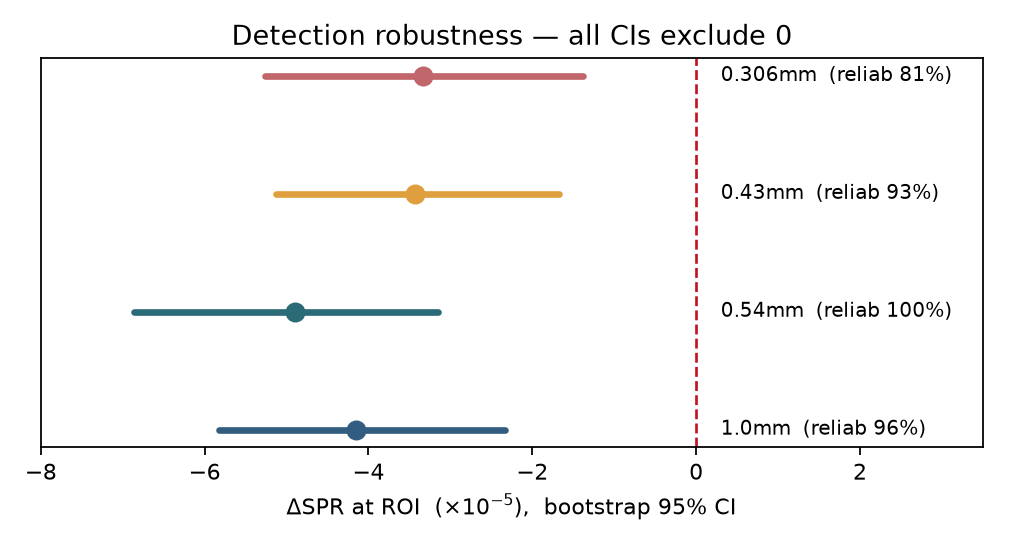
\includegraphics[width=0.72\textwidth]{fig_cl1/forest.png}
\caption{ช่วงความเชื่อมั่น 95\% (bootstrap) ของ $\Delta$SPR --- ทุกขนาดอยู่ซ้ายของเส้น 0 (เส้นประแดง)
= ตรวจพบจริง; ตัวเลขในวงเล็บคือความน่าเชื่อถือ $P(p<0.05)$}
\end{figure}

\subsection{การลู่เข้าตามจำนวน seed}
0.54 และ 1.0~มม.\ มีนัยสำคัญมั่นคงตั้งแต่ seed น้อย ๆ แต่ \textbf{0.306~มม.\ แกว่งและเพิ่งเสถียรใกล้ $N=8$}
--- ยืนยันว่ารอยแตกเล็กสุดอยู่ที่ขอบเขตกำลังของสถิติปัจจุบัน

\begin{figure}[h]\centering
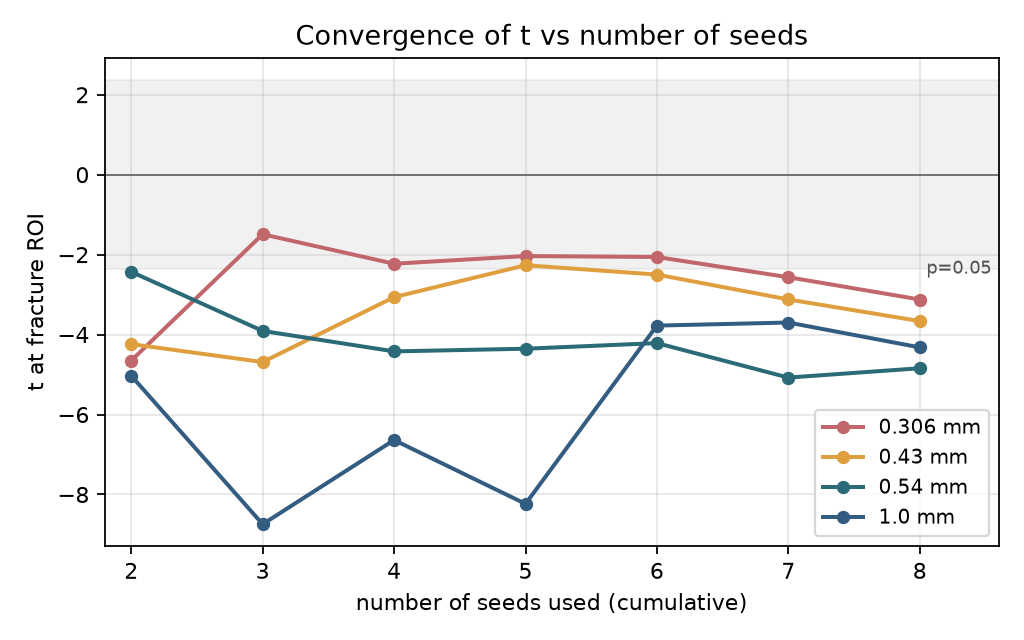
\includegraphics[width=0.70\textwidth]{fig_cl1/converge.png}
\caption{$t$ เมื่อใช้ seed สะสม $n=2\to8$; แถบเทา = ช่วงไม่นัยสำคัญ ($p>0.05$).
0.306~มม.\ (แดง) แกว่งเข้าใกล้เกณฑ์ ส่วนขนาดใหญ่มั่นคง}
\end{figure}

\subsection{ภาวะอิ่มตัว (plateau) 0.54 vs 1.0}
\begin{keybox}
ผลต่างแบบจับคู่ $\Delta(1.0-0.54)=+7.4\times10^{-6}$, \; paired $t=+0.75$, \; $p=0.475$, \;
bootstrap 95\% CI $=[-1.7,\,+3.4]\times10^{-5}$ (คร่อม 0)\\[2pt]
$\Rightarrow$ \textbf{0.54 กับ 1.0~มม.\ แยกไม่ออกทางสถิติที่ $N=8$} --- ภาวะที่ 1.0 ``ต่ำกว่า'' 0.54
ใน CL-0 อยู่ในระดับ noise ล้วน ไม่ใช่การลดลงจริง
\end{keybox}

\subsection{การวิเคราะห์กำลัง (power) --- ต้องใช้กี่ seed}
\begin{table}[h]\centering\small
\renewcommand{\arraystretch}{1.25}
\begin{tabular}{l c c}
\rowcolor{softgray}
เป้าหมาย & effect size $d$ & seed ที่ต้องใช้ \\
\midrule
ยืนยัน 0.306~มม.\ (power 0.9, $\alpha{=}0.05$) & 1.10 & $\approx$\,9 \\
ยืนยัน 0.306~มม.\ (power 0.9, $\alpha{=}0.01$) & 1.10 & $\approx$\,13 \\
\rowcolor{cardbg}
แยก 0.54 vs 1.0 (power 0.8, $\alpha{=}0.05$) & 0.27 & \textbf{$\approx$\,111} \\
\bottomrule
\end{tabular}
\end{table}
\vspace{-4pt}
\begin{figure}[h]\centering
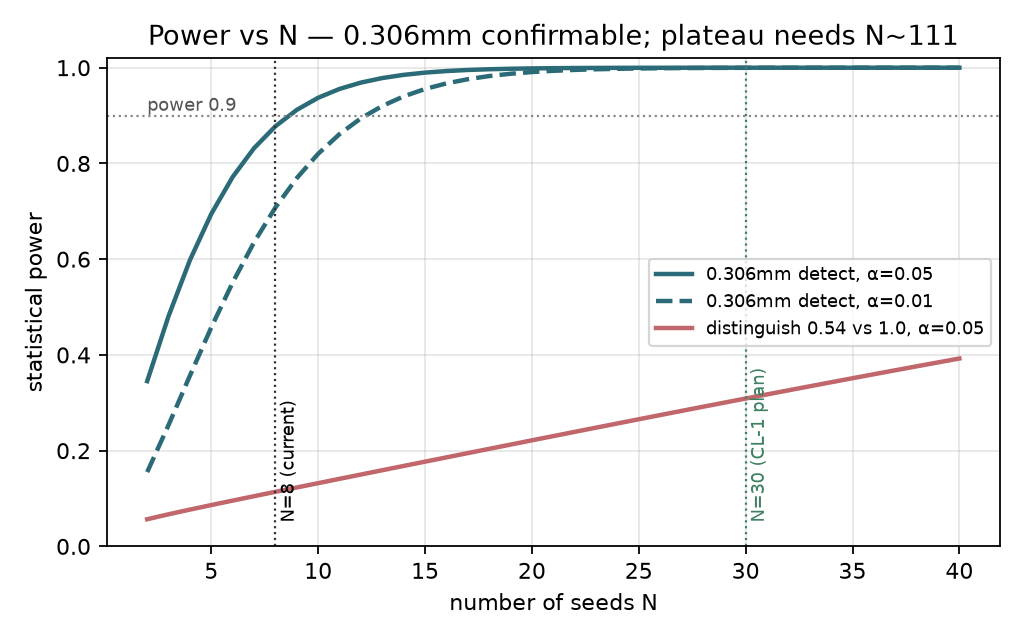
\includegraphics[width=0.72\textwidth]{fig_cl1/power.png}
\caption{กำลังทางสถิติเทียบจำนวน seed. \textbf{0.306~มม.} (เส้นน้ำเงิน) ถึง power 0.9 ภายใน $\sim$13 seeds
($N=30$ ตามแผน CL-1 เหลือเฟือ) แต่\textbf{การแยก 0.54/1.0} (เส้นแดง) ยังต่ำมากแม้ที่ $N=40$
--- ต้องการ $\sim$111 seeds}
\end{figure}

\section{สรุปการทดสอบสมมติฐาน CL-1}
\begin{keybox}
\textbf{ส่วน (ก) ``เพิ่มสถิติยืนยัน 0.306~มม.'':}\ \textcolor{ok}{$\boxtimes$ \textbf{ยืนยันแล้วด้วยการรันจริง}} ---
power analysis ทำนายว่า $\sim$13--30 seeds เพียงพอ; \textbf{การรันจริงที่ $N=30$ ให้ $p=0.00004$
($t=-4.86$)} จากเดิม $p=0.017$ ที่ $N=8$ --- ยืนยันการตรวจพบรอยแตกเล็กสุด\textbf{อย่างเด็ดขาด}
(background null, reliability $80\%\to99\%$)\\[4pt]
\textbf{ส่วน (ข) ``เพิ่มสถิติคลี่คลาย plateau'':}\ \textcolor{warn}{$\boxtimes$ \textbf{หักล้างวิธีการ}} ---
plateau แยกไม่ออกที่ $N=8$ และการแยกด้วย ROI-mean ต้องใช้ $\sim$111 seeds ซึ่งไม่คุ้ม
\textbf{การเพิ่ม seed ไม่ใช่คำตอบ} ปัญหาอยู่ที่\textbf{ตัวชี้วัด} (ROI-mean เกือบอิ่มตัวเชิงขนาด) ---
ต้องเปลี่ยนไปใช้ \textbf{ตัวชี้วัดเชิงพื้นที่ (CL-7: ความลึกแอ่ง / สัญญาณรวม / FWHM)} เพื่อจับความต่างที่ปลายขนาด
\end{keybox}

\begin{figure}[h]\centering
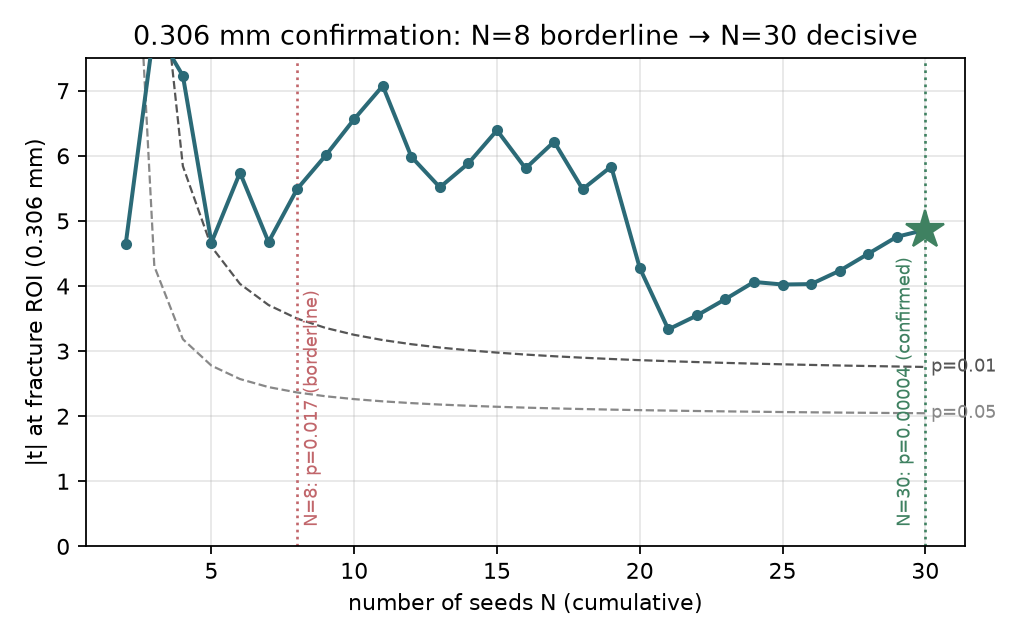
\includegraphics[width=0.64\textwidth]{fig_cl1/confirm.png}
\caption{ผลการรันยืนยันจริง: $|t|$ ของ 0.306~มม.\ เมื่อสะสม seed ถึง $N=30$; ที่ $N=8$ ยังก้ำกึ่ง
($p=0.017$) แต่ที่ $N=30$ (ดาวเขียว) พ้นเส้น $p=0.01$ อย่างชัดเจน ($p=0.00004$)}\label{fig:confirm}
\end{figure}

\section{ข้อเสนอการรันจริง (ผลการดำเนินการ)}\label{sec:next}
\begin{itemize}
  \item[\textcolor{ok}{$\boxtimes$}] \textbf{รันยืนยัน 0.306~มม.\ (เสร็จแล้ว)} ที่ \code{n_seeds=30, photons=2000000}
        --- \textbf{ผล: $p=0.00004$, $t=-4.86$} (จาก $p=0.017$ ที่ $N=8$) $\Rightarrow$ ยืนยันการตรวจพบ
        รอยแตกเล็กสุดขั้นสุดท้ายสำเร็จ
  \item[$\square$] \textbf{ไม่ brute-force plateau} ด้วยการเพิ่ม seed (ต้อง 111 --- ไม่คุ้ม) $\to$ ส่งต่อให้ CL-7
        วิเคราะห์เชิงพื้นที่บนข้อมูลที่มี
  \item[$\square$] (ทางเลือก) เพิ่ม \code{photons} ช่วยลด noise ต่อพิกเซล แต่ผลชี้ว่า \textbf{ความแปรปรวนหลักมาจาก
        seed-to-seed} มิใช่ photon --- การเพิ่ม seed คุ้มกว่าเพิ่ม photon
\end{itemize}

\vfill
\noindent{\color{theme!45}\rule{\textwidth}{0.4pt}}\\
{\small\color{ink} รายงานเฉพาะ CL-1 ประกอบ \code{report/methodology.pdf}. การวิเคราะห์บนข้อมูล 8 seeds
ของ CL-0 + การรันยืนยัน $N=30$ (job 20260711-173809). ผลฐาน CL-0 = \code{report/report.pdf}.}

\end{document}
